Defining \acrfull{vr} and showing the main charactristics of it through this chapter. Followed by listing a number of related projects that has been made in Palestine to represent the country. The last section will represent example projects that has been done in \acrshort{vr} in different places in the world.  
\section{Virtual Reality} 
Virtual reality is a technology which is often regarded as a natural extension to 3D computer graphics with advanced input and output devices \citep{Jayaram1997}. Ryan (2001) defined it as an “interactive, immersive experience generated by a computer” \citep{Ryan2001}. And according to G.C. Burdea and Coiffet (2017) “it is a generated computer graphics used to create a realistic-looking world that responds to the user’s input (gestures, verbal commands, etc.)” \cite[p.20]{burdea2017virtual}. Virtual reality places the users inside the experience instead of viewing a screen in front of them, the users will be immersed inside a 3D world.“The scientific community has been working in the field of virtual reality (VR) for decades, having recognized it as a very powerful human-computer interface”\cite[p.19]{burdea2017virtual} As shown in Figure \ref{fig:3I} Three elements are needed to construct a virtual reality situation: immersion, interaction, and imagination. They are called the “3I’s” of virtual reality \citep{Hu2016,burdea2017virtual}.




1. \textbf{Immersion:} it is the virtual reality situation where the user feels personally inside the
scene and immerse inside the simulated virtual world.



2. \textbf{Interaction:} The interactive feedback between the user
and the virtual environment. Since it is a man-machine
interface, the system should promptly respond to the
user’s actions.


\begin{wrapfigure}{r}{0.30\textwidth} %this figure will be at the left
    \centering
    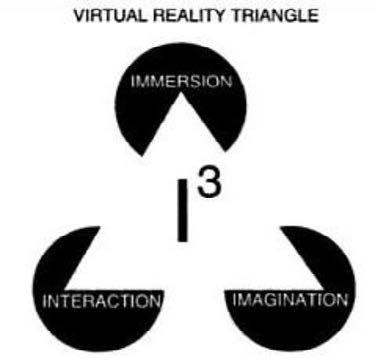
\includegraphics[width=0.30\textwidth]{3I}
    \caption{The 3I's of Virtual Reality - © 2003 by John Wiley \& Sons Inc. All rights
reserved}
    \label{fig:3I}
\end{wrapfigure}

3. \textbf{Imagination:} The scene design and the construction of
the environment formulated with imagination for a
better user simulated experience.


Emotional and physical reaction would be caused to the user due to a strong mediated presence as if the virtual world existed physically, the impression of being in a real place, as well as plausibility illusion, having the sensation that the scenario being depicted is actually occurring. Those illusions occur despite the fact that the user is aware that the virtual world is only a simulation. \acrshort{vr} is one of the main trends in the evolution of presence \citep{Waterworth2014, Steinicke2016}.
The Human-computer interaction is extended from purely visual interaction to diversified interaction that the user could interact with objects in virtual reality with the perceived experiences and cognitive processing abilities as in the real world, and the feeling is close to the changes in the natural world \citep{Hu2016}. One of the ways of interactions is the user's gaze determines the direction and clicking a button on the mouse moves the user forward. The mouse can also lift and move objects in the virtual environment. When the user collides with an object, a mouse button is pushed to lift it and the object then moves with the user until a button is pushed to drop it \citep{Aguinas2004}.




  
  
  
  
  
\section{Related Work}
\section{Example projects}
\textbf{Auschwitz Virtual Tour}\footnote{Auschwitz VR Tour-\url{https://youtu.be/EOM_CxAKB_Y}}: The German broadcasting institution WDR made a 360o
documentary in Auschwitz concentration camp. Within the documentary, some Holocaust
survivors tell their stories. While listening to the stories and seeing the different locations in
the camp the user could feel the fear and horror that people suffered from. The video
immerses the user through the sound of the surrounding environment in the camp, you can
hear the wind and the sound gives a slight feeling of the cold weather over there. The
experience is immersive, but there is no interactivity with the user.


\textbf{Clouds over Sidra}\footnote{The Za’atari camp VR Tour-\url{https://youtu.be/mUosdCQsMkM}}: A 12 years old girls’ daily life story at the Za’atari refugee camp in Jordan
showed in virtual reality. The camp is a home for 80,000 Syrian refugees, half of them are
children(“Syrian Refugee Crisis – UN Virtual Reality,” 2015). The documentary was made by
the United Nation to raise awareness about the Syrian crisis. The video contained a number
of short videos from different parts of the camp, and it’s being synchronized while Sidra
narrates her story. It is more like watching a video with empathy than being immersed, but
the video presents the real life of the camp. Although the difference that while watching and
listening to the story, the user observes the people how they actually survive and live in the
camp. Therefore, the user does not have to imagine how is life over there.


\textbf{Carne y arena}\footnote{Carne y Arena Trailer-\url{https://youtu.be/zF-focK30WE}} : A highly professional
Virtual reality project that puts viewers
into the harsh life of an immigrant. The
user is placed among a group of
Mexican immigrants passing the
borders into the U.S. It was written and
directed by Alejandro G. Iñárritu. It Is a
full virtual reality experience; the user
needs to reserve an individual session
on the website. According to Pinotti (2017) you go in a dark room; your feet are on the sand (coarse grain, rough feeling) then, two assistants welcome you and provide you with the
necessary devices: an Oculus Rift headset, a backpack connected via cables to a powerful
computer and you are ready to be caught up in a nightmare \citep{Pinotti2017}. The project is
subtitled by ‘Virtually present, Physically invisible’. Pinotti (2017) defined, Virtually present:
“you are transported in the middle of the desert, among men, women, and children who try
their voyage of hope”. Physically invisible: “you are present, but nobody sees you and after a
while, you start to feel the need to be noticed and seek acknowledgment of social
recognition” \citep{Pinotti2017}. The project was developed with high technology, like 3D
modeling, visual effects, sound. The interaction of the user and the feeling of “being there”
by placing the user in a special environment, leads to a unique experience of immersion.


